\documentclass[12pt, letterpaper]{article}
\AtBeginDocument{\nocite{*}}
\usepackage{graphicx}
\usepackage{amsmath} 
\usepackage{booktabs}
\usepackage{multirow} 
\usepackage{caption}
\usepackage{subcaption}
\usepackage{float}
\usepackage{csvsimple}
\usepackage{tabularx}
\usepackage{siunitx}
\usepackage{textcomp}
\usepackage{pythonhighlight}
\usepackage[a4paper, total={6in, 8in}]{geometry}
\usepackage{etoolbox}
\usepackage{microtype} % Improves typography and reduces overfull boxes
\usepackage{seqsplit}  % For splitting long sequences
\usepackage{ragged2e} 
\usepackage[T1]{fontenc} % Essential for European characters
\usepackage{textcomp} % For additional symbols
\usepackage{upquote} % For straight quotes in verbatim
\restylefloat{table}
\usepackage{minted}
\usepackage{comment}
\usepackage{hyperref}  % Allows \url{} and clickable links
\usepackage{gensymb}
\usepackage{bm}
\usepackage{braket}

\setminted{
    breaklines=true,
    breaksymbolleft=,
    fontsize=\small
}

\AtBeginDocument{\RenewCommandCopy\qty\SI}


\title{Lab 5: Lasers and LEDs}
\author{Mathilde DECLERCQ - 123700659}
\begin{document}
\maketitle
\newpage

\pagenumbering{Roman}
\tableofcontents
\pagenumbering{arabic}
\setcounter{page}{1} 
\newpage

\section{Introduction}
The purpose of this two-weeks lab is to characterise the LIV (Light, Current, Voltage) properties of a red laser and multiple different colours of LEDs. For that we will use the current source built in Lab 2 and the photoreceiver that converts light into voltage from Lab 4. Prior to this lab a laser safety lecture has been given to manipulate the laser used in this lab safely.

\section{Pre - Lab}
Laser informations from the spec sheet:
\begin{itemize}
    \item $\lambda$ = $650~\mathrm{nm}$
    \item P = $5~\mathrm{mW}$, here we will take P = $7~\mathrm{mW}$ to ensure the validity of our calculations
    \item Divergences angles: $\theta_{\parallel } = 6 ^{\circ} = 0.104 ~\mathrm{rad}$ and $\theta_{\perp } = 24^{\circ} = 0.409~\mathrm{rad}$
\end{itemize}
\subsection{In Lab}
\subsubsection*{MPE}
For $t=0.25s$:
\[
MPE = 18\times t^{0.75} ~\mathrm{Jm^{-2}}
\]
\[
MPE = 18\times 0.25^{0.75}  = 6.36 ~\mathrm{Jm^{-2}}
\]
\[
MPE = 25.5 ~\mathrm{Wm^{-2}}
\]
\subsubsection*{AEL}
\[
AEL = MPE \times Area 
\]
\[
AEL = 25.5 \pi \left( \frac{0.007}{2} \right)^{2} \approx 1~\mathrm{mW}
\]
\subsubsection*{NOHD}
\[
NOHD = 2 \sqrt{\frac{P}{MPE\times\pi\left(\theta\right)^{2}}}
\]
\[
NOHD = 2 \sqrt{\frac{7\times10^{-3}}{\left(25.5\right)\times\pi\left(0.419\right)\left(0.104\right)}} \approx 0.09~\mathrm{m}
\]
\[
NOHD = 9~\mathrm{cm}
\]
\subsection{Class 1}
\subsubsection*{MPE}
For $t=30000s$:\\
From Table A.1:
\[
MPE = 10 ~\mathrm{Wm^{-2}}
\]
\subsubsection*{AEL}
\[
AEL = MPE \times Area 
\]
\[
AEL = 10 \pi \left( \frac{0.007}{2} \right)^{2} \approx 4 \times 10^{-4}~\mathrm{W}
\]
\subsubsection*{NOHD}
\[
NOHD = 2 \sqrt{\frac{P}{MPE\times\pi\left(\theta\right)^{2}}}
\]
\[
NOHD = 2 \sqrt{\frac{7\times10^{-3}}{\left(10\right)\times\pi\left(0.419\right)\left(0.104\right)}} =0.143~\mathrm{m}
\]
\[
NOHD = 15~\mathrm{cm}
\]

\subsection{Current range}

From the spec sheet, the current range for the AlGnInP laser is $0\mathrm{mA} \geq I \geq 35 \mathrm{mA}$. For relevance, the same current range will be used for LEDs.

\subsection{Design of the circuits}
For this circuit, the OpAmp MCP601 has been used and it has been powered up with a dual power supply of $+5V$ and $0V$. The diagram of the circuit is shown below:

\begin{figure}[H]
    \centering
    \begin{subfigure}{0.49\textwidth}
        \includegraphics[width = \textwidth]{photoreceiver_scheme.png}
        \subcaption{Photoreceiver circuit diagram}
        \label{fig:photoreceiver}     
    \end{subfigure}
    \hfil
    \begin{subfigure}{0.49\textwidth}
        \includegraphics[width = \textwidth]{2_4_wire_scheme.png}
        \subcaption{2 and 4 wire circuit diagram}
        \label{fig:2_4}
    \end{subfigure}
        
    \caption{Circuit diagrams}
    \label{fig:diagrams}
\end{figure}
The value of the feedback resistor $R_{f}$ is chosen to be $26.7\mathrm{k\Omega}$  and the protection resistance is $R_{p} = 2.17\mathrm{k\Omega}$. For the resistance used in the 2 and 4 wire circuit, their values is $R = 2.2\mathrm{k\Omega}$.

\section{Lab results}
The pictures of the experimental setup can be found below:
\begin{figure}[H]
    \centering
    \begin{subfigure}{0.49\textwidth}
        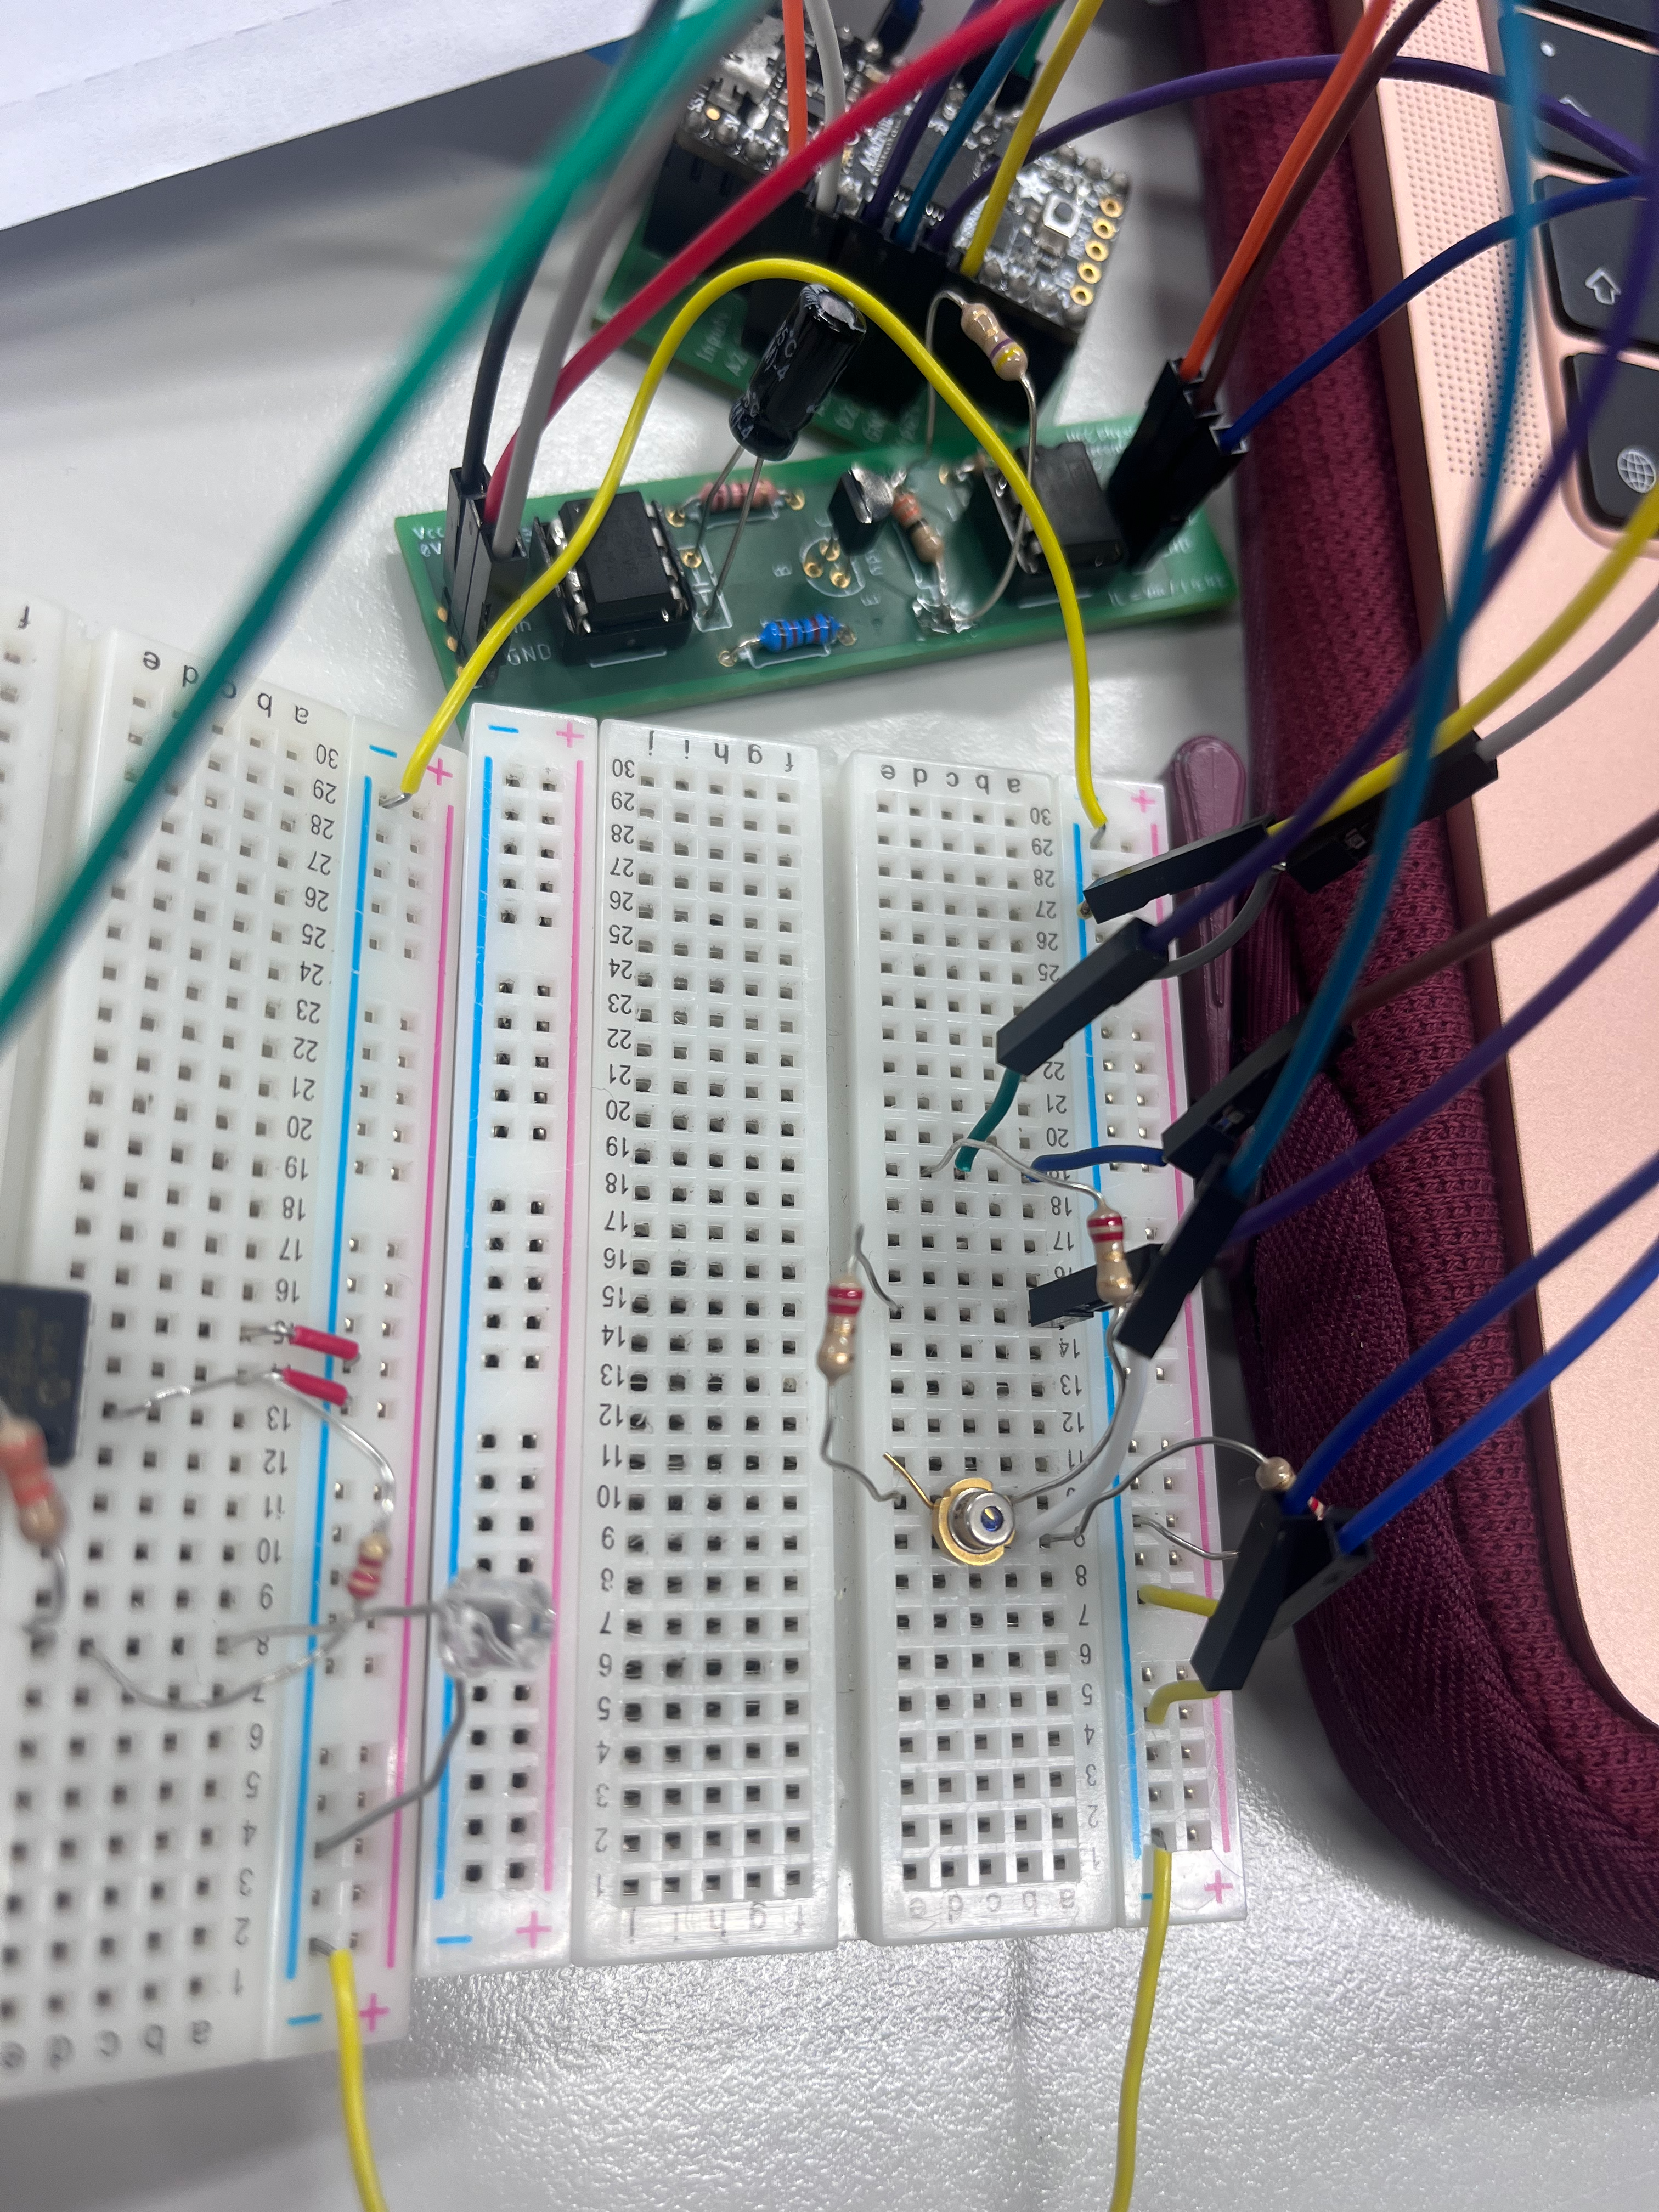
\includegraphics[width = \textwidth]{IMG_3154.png}
        \subcaption{Photoreceiver circuit for the laser}
        \label{fig:photoreceiver_laser}     
    \end{subfigure}
    \hfil
    \begin{subfigure}{0.49\textwidth}
        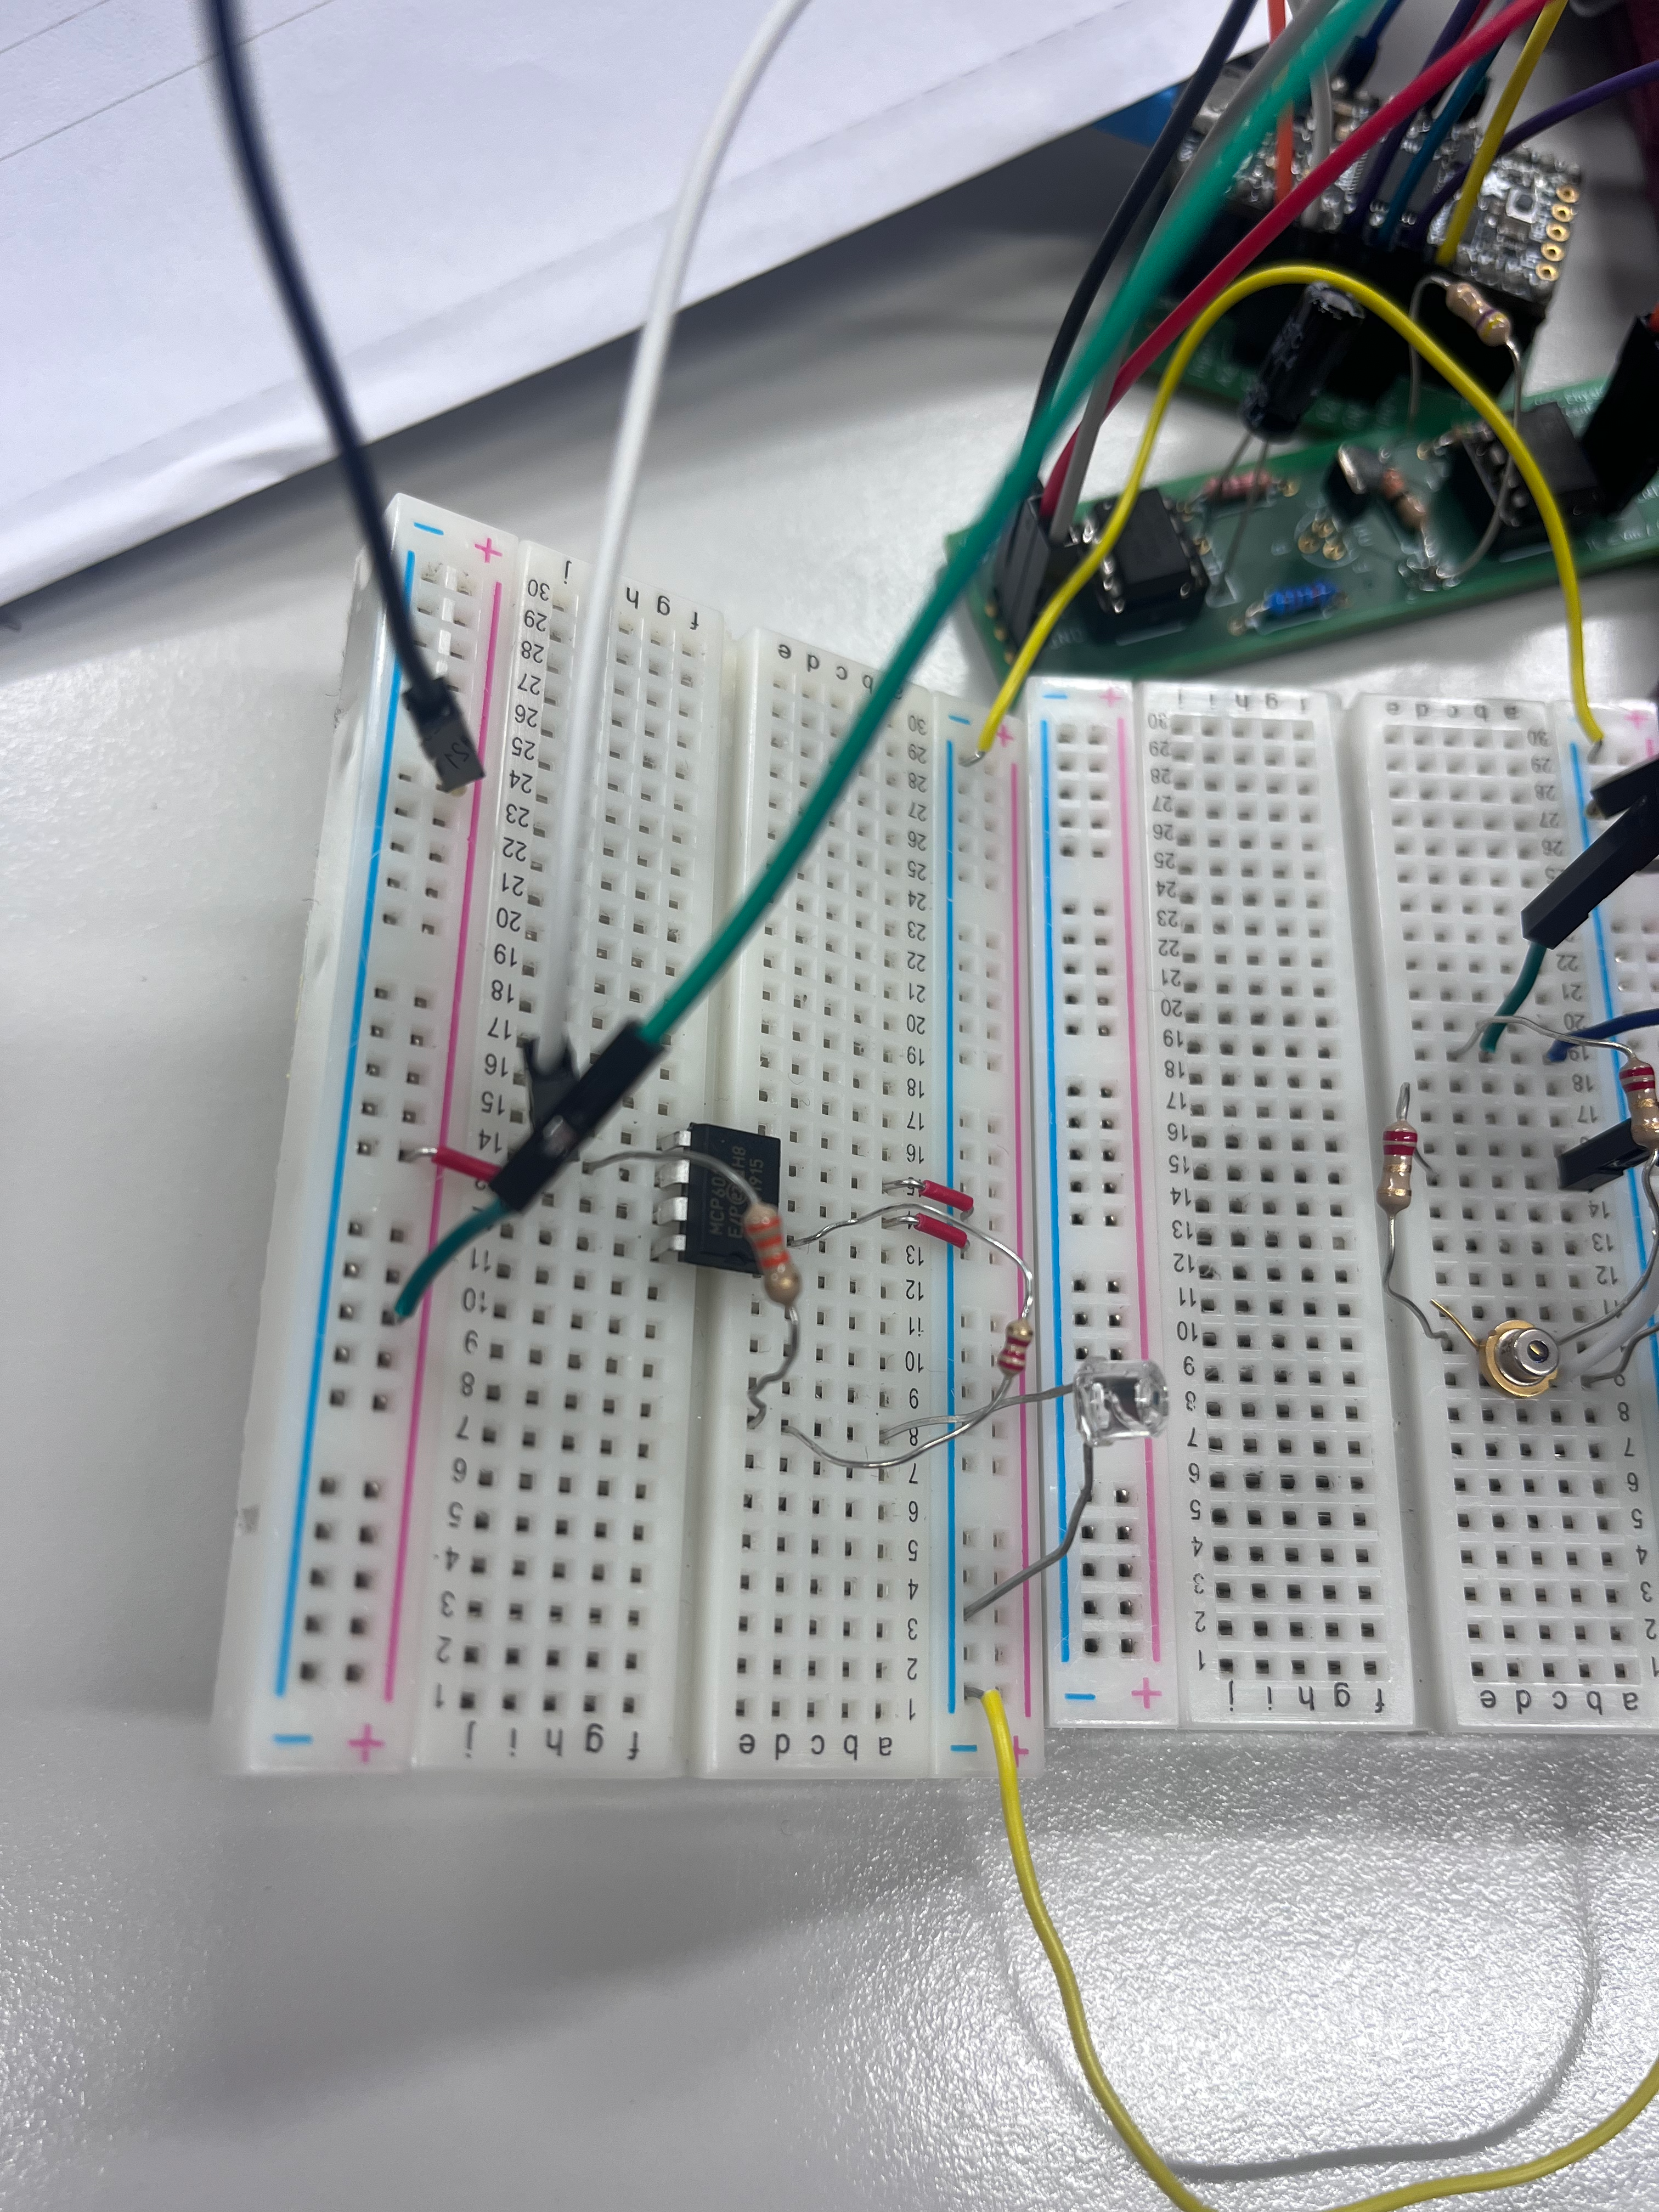
\includegraphics[width = \textwidth]{IMG_3155.png}
        \subcaption{2 and 4 wire circuit diagram}
        \label{fig:2_4_photodiode}
    \end{subfigure}
        
    \caption{Circuit setup}
    \label{fig:setup}
\end{figure}
A different photodiode then the SFH 203 P has been used for data collection of the laser.\\
To calculate the optical power, the following formula has been used:
\[
P = \frac{V_{out}}{G \times R_{\lambda}}
\]
Where $V_{out}$ is the output voltage of the photoreceiver circuit, $G$ is the transimpedance gain in $\mathrm{V/A}$, $R_{\lambda}$ is photodiode responsivity in $\mathrm{V/A}$ at laser wavelength. For the red laser at $650\mathrm{nm}$, $R_{\lambda} = 0.4 \mathrm{A/W}$. 
\subsection{IV characterisation}
The data sheets for each devices can be found in the Appendix.

\subsubsection{Red LED}
\begin{figure}[H]
    \centering
    \includegraphics[width=\textwidth]{commands/IV_LI_Characteristics_red.png}
    \caption{Red LED IV curve with logarithmic fit and optical power.}
    \label{fig:red.1}
\end{figure}

The Figure~\ref{fig:red.1} shows both 2 and 4-wire measurements with their logarithmic fits, as well as the optical power in $\mathrm{\mu W}$. 

\subsubsection*{Observations:}

\begin{itemize}
    \item Optical Power: 
    \begin{itemize}
        \item Slope with logarithmic form.
        \item No irregularities in the data.
        \item Reaches a maximum of $30\mathrm{\mu W}$ at $35\mathrm{mA}$.
    \end{itemize}
    \item The 2-wire measurement has a logarithmic fit of $V = 0.223 \ln(I) + 1.640$.
    \item The 4-wire measurement has a logarithmic fit of $V = 0.188 \ln(I) + 1.636$. 
\end{itemize}


Alternative view of the IV curve for the 2 and 4-wire measurements:
\begin{figure}[H]
    \centering
    \begin{subfigure}{\textwidth}
        \centering
        \includegraphics[width=0.8\textwidth]{commands/Device_2_4_wire_Characterization_red.png}
        \subcaption{V-I curve of the photodiode lit up by a red LED with a zoom on the 2 and 4-wire measurements for a current range of $15-35\mathrm{mA}$}
        \label{fig:red.3}
    \end{subfigure}
    
    \vspace{1em} % Optional spacing between subfigures

    \begin{subfigure}{\textwidth}
        \centering
        \includegraphics[width=0.8\textwidth]{commands/Device_Resistance_Characterization_red.png}
        \subcaption{Resistance comparison for data extraction for the red LED zoomed in for a current range of $15-35\mathrm{mA}$}
        \label{fig:red.4}
    \end{subfigure}

    \caption{Red LED results: (a) V-I curve with zoom on 2- and 4-wire measurements; (b) resistance comparison for data extraction.}
    \label{fig:red.combined}
\end{figure}

\subsubsection*{Observations}

Figure~\ref{fig:red.combined} shows that the resistance of the amber LED depends on the current. According to Figure~\ref{fig:red.3}, the 2-wire slope is $V = 0.0193 (I) + 1.895$, while the 4-wire slope is $V = 0.0146 (I) + 1.885$. The resistance can be extracted from the slope as $R = \frac{\Delta V}{\Delta I}$. Therefore, the resistance for the 2-wire measurement is $R_{2-wire} = 19.3 \mathrm{\Omega}$ and for the 4-wire measurement is $R_{4-wire} = 14.6 \mathrm{\Omega}$. The internal resistance of the circuit can be calculated as $R_{circuit} = R_{2-wire} - R_{4-wire} = 4.6 \mathrm{\Omega}$. The internal resistance of the circuit is responsible for the difference in slopes, where the lead resistance and contact resistances are significantly affecting the 2-wire results.

Figure~\ref{fig:red.4} shows how the voltage drops across the resistors in the circuit.

\subsubsection{Amber LED}
\begin{figure}[H]
    \centering
    \includegraphics[width=\textwidth]{commands/IV_LI_Characteristics_amber.png}
    \caption{Amber LED IV curve with logarithmic fit and optical power.}
    \label{fig:amber.1}
\end{figure}

The Figure~\ref{fig:amber.1} shows both 2 and 4-wire measurements with their logarithmic fits, as well as the optical power in $\mathrm{\mu W}$. 


\subsubsection*{Observations:}

\begin{itemize}
    \item Optical Power: 
    \begin{itemize}
        \item Slope with linear form.
        \item No irregularities in the data.
        \item Reaches a maximum of $\approx 32\mathrm{\mu W}$ at $35\mathrm{mA}$.
    \end{itemize}
    \item The 2-wire measurement has a logarithmic fit of $V = 0.152 \ln(I) + 1.625$.
    \item The 4-wire measurement has a logarithmic fit of $V = 0.116 \ln(I) + 1.626$. 
\end{itemize}

Alternative view of the IV curve for the 2 and 4-wire measurements:
\begin{figure}[H]
    \centering
    \begin{subfigure}{\textwidth}
        \centering
        \includegraphics[width=0.8\textwidth]{commands/Device_2_4_wire_Characterization_amber.png}
        \subcaption{V-I curve of the photodiode lit up by an amber LED with a zoom on the 2 and 4-wire measurements for a current range of $15-35\mathrm{mA}$}
        \label{fig:amber.3}
    \end{subfigure}
    
    \vspace{1em} % Optional spacing between subfigures

    \begin{subfigure}{\textwidth}
        \centering
        \includegraphics[width=0.8\textwidth]{commands/Device_Resistance_Characterization_amber.png}
        \subcaption{Resistance comparison for data extraction for the amber LED zoomed in for a current range of $15-35\mathrm{mA}$}
        \label{fig:amber.4}
    \end{subfigure}

    \caption{Amber LED results: (a) V-I curve with zoom on 2- and 4-wire measurements; (b) resistance comparison for data extraction.}
    \label{fig:amber.combined}
\end{figure}

\subsubsection*{Observations}

Figure~\ref{fig:amber.combined} shows that the resistance of the amber LED depends on the current. According to Figure~\ref{fig:amber.3}, the 2-wire slope is $V = 0.0077 (I) + 1.910$, while the 4-wire slope is $V = 0.0030 (I) + 1.901$. The resistance can be extracted from the slope as $R = \frac{\Delta V}{\Delta I}$. Therefore, the resistance for the 2-wire measurement is $R_{2-wire} = 7.7 \mathrm{\Omega}$ and for the 4-wire measurement is $R_{4-wire} = 3.0 \mathrm{\Omega}$. The internal resistance of the circuit can be calculated as $R_{circuit} = R_{2-wire} - R_{4-wire} = 4.3 \mathrm{\Omega}$. The internal resistance of the circuit is responsible for the difference in slopes, where the lead resistance and contact resistances are significantly affecting the 2-wire results.

Figure~\ref{fig:amber.4} shows how the voltage drops across the resistors in the circuit.


\subsubsection{Green LED}
\begin{figure}[H]
    \centering
    \includegraphics[width=\textwidth]{commands/IV_LI_Characteristics_green.png}
    \caption{Green LED results IV curve with logarithmic fit and optical power.}
    \label{fig:green.1}
\end{figure}

The Figure~\ref{fig:green.1} shows both 2 and 4-wire measurements with their logarithmic fits, as well as the optical power in $\mathrm{\mu W}$. 


\subsubsection*{Observations:}

\begin{itemize}
    \item Optical Power: 
    \begin{itemize}
        \item Slope with linear form.
        \item No irregularities in the data.
        \item Reaches a maximum of $\approx 34\mathrm{\mu W}$ at $35\mathrm{mA}$.
    \end{itemize}
    \item The 2-wire measurement has a logarithmic fit of $V = 0.264 \ln(I) + 1.646$.
    \item The 4-wire measurement has a logarithmic fit of $V = 0.222 \ln(I) + 1.660$. 
\end{itemize}


Alternative view of the IV curve for the 2 and 4-wire measurements:
\begin{figure}[H]
    \centering
    \begin{subfigure}{\textwidth}
        \centering
        \includegraphics[width=0.8\textwidth]{commands/Device_2_4_wire_Characterization_green.png}
        \subcaption{V-I curve of the photodiode lit up by a green LED with a zoom on the 2 and 4-wire measurements for a current range of $15-35\mathrm{mA}$}
        \label{fig:green.3}
    \end{subfigure}
    
    \vspace{1em} % Optional spacing between subfigures

    \begin{subfigure}{\textwidth}
        \centering
        \includegraphics[width=0.8\textwidth]{commands/Device_Resistance_Characterization_green.png}
        \subcaption{Resistance comparison for data extraction for the green LED zoomed in for a current range of $15-35\mathrm{mA}$}
        \label{fig:green.4}
    \end{subfigure}

    \caption{Green LED results: (a) V-I curve with zoom on 2- and 4-wire measurements; (b) resistance comparison for data extraction.}
    \label{fig:green.combined}
\end{figure}

\subsubsection*{Observations}

Figure~\ref{fig:green.combined} shows that the resistance of the green LED depends on the current. According to Figure~\ref{fig:green.3}, the 2-wire slope is $V = 0.0229 (I) + 1.946$, while the 4-wire slope is $V = 0.0181 (I) + 1.937$. The resistance can be extracted from the slope as $R = \frac{\Delta V}{\Delta I}$. Therefore, the resistance for the 2-wire measurement is $R_{2-wire} = 22.9 \mathrm{\Omega}$ and for the 4-wire measurement is $R_{4-wire} = 18.1 \mathrm{\Omega}$. The internal resistance of the circuit can be calculated as $R_{circuit} = R_{2-wire} - R_{4-wire} = 4.8 \mathrm{\Omega}$. The internal resistance of the circuit is responsible for the difference in slopes, where the lead resistance and contact resistances are significantly affecting the 2-wire results.

Figure~\ref{fig:green.4} shows how the voltage drops across the resistors in the circuit.

\subsubsection{Blue LED}
\begin{figure}[H]
    \centering
    \includegraphics[width= \textwidth]{commands/IV_LI_Characteristics_blue.png}
    \caption{Blue LED results IV curve with logarithmic fit and optical power.}
    \label{fig:blue.1}
\end{figure}

The Figure~\ref{fig:blue.1} shows both 2 and 4-wire measurements with their logarithmic fits, as well as the optical power in $\mathrm{\mu W}$. 

\subsubsection*{Observations:}

\begin{itemize}
    \item Optical Power: 
    \begin{itemize}
        \item Slope with logarithmic form.
        \item No irregularities in the data.
        \item Reaches a maximum of $\approx 85\mathrm{\mu W}$ at $35\mathrm{mA}$.
    \end{itemize}
    \item The 2-wire measurement has a logarithmic fit of $V = 0.294 \ln(I) + 2.329$.
    \item The 4-wire measurement has a logarithmic fit of $V = 0.267 \ln(I) + 2.325$. 
\end{itemize}

Alternative view of the IV curve for the 2 and 4-wire measurements:
\begin{figure}[H]
    \centering
    \begin{subfigure}{\textwidth}
        \centering
        \includegraphics[width=0.8\textwidth]{commands/Device_2_4_wire_Characterization_blue.png}
        \subcaption{V-I curve of the photodiode lit up by a blue LED with a zoom on the 2 and 4-wire measurements for a current range of $15-35\mathrm{mA}$}
        \label{fig:blue.3}
    \end{subfigure}
    
    \vspace{1em} % Optional spacing between subfigures

    \begin{subfigure}{\textwidth}
        \centering
        \includegraphics[width=0.8\textwidth]{commands/Device_Resistance_Characterization_blue.png}
        \subcaption{Resistance comparison for data extraction for the blue LED zoomed in for a current range of $15-35\mathrm{mA}$}
        \label{fig:blue.4}
    \end{subfigure}

    \caption{Blue LED results: (a) V-I curve with zoom on 2- and 4-wire measurements; (b) resistance comparison for data extraction.}
    \label{fig:blue.combined}
\end{figure}

\subsubsection*{Observations}

Figure~\ref{fig:blue.combined} shows that the resistance of the blue LED depends on the current. According to Figure~\ref{fig:blue.3}, the 2-wire slope is $V = 0.0091 (I) + 3.037$, while the 4-wire slope is $V = 0.0104 (I) + 2.912$. The resistance can be extracted from the slope as $R = \frac{\Delta V}{\Delta I}$. Therefore, the resistance for the 2-wire measurement is $R_{2-wire} = 9.1 \mathrm{\Omega}$ and for the 4-wire measurement is $R_{4-wire} = 10.4 \mathrm{\Omega}$. The internal resistance of the circuit can be calculated as $R_{circuit} = R_{2-wire} - R_{4-wire} = -0.9 \mathrm{\Omega}$. The internal resistance of the circuit is negative, which is not physically possible. This discrepancy may be due to measurement errors or variations in the LED's characteristics. The internal resistance of the circuit is responsible for the difference in slopes, where the lead resistance and contact resistances are significantly affecting the 2-wire results.

Figure~\ref{fig:blue.4} shows how the voltage drops across the resistors in the circuit.

\subsubsection{Laser}
\begin{figure}[H]
    \centering
    \includegraphics[width = 0.8\textwidth]{commands/IV_LI_Characteristics_Laser.png}
    \caption{Laser results IV curve with logarithmic fit and optical power.}
    \label{fig:laser.1}
\end{figure}

The Figure \ref{fig:laser.1} shows both 2 and 4-wire measurements with their logarithmic fits, as well as the optical power in $\mathrm{\mu W}$. 

\subsubsection*{Observations:}

\begin{itemize}
    \item Optical Power: 
    \begin{itemize}
        \item Slope with linear form.
        \item Irregularities in the data, with a peak at \(0.2\mathrm{mA}, 0.9 \mathrm{\mu W}\)
        \item Reaches a maximum of $0.53\mathrm{\mu W}$ at $35\mathrm{mA}$.
    \end{itemize}
    \item The 2-wire measurement has a logarithmic fit of $V = 0.363 \ln(I) + 1.177$.
    \item The 4-wire measurement has a logarithmic fit of $V = 0.317 \ln(I) + 1.205$. 
\end{itemize}

Alternative view of the IV curve for the 2 and 4-wire measurements:
\begin{figure}[H]
    \centering
    \begin{subfigure}{\textwidth}
        \centering
        \includegraphics[width=0.8\textwidth]{commands/Device_2_4_wire_Characterization_laser.png}
        \subcaption{V-I curve of the photodiode lit up by a laser with a zoom on the 2 and 4-wire measurements for a current range of $15-35\mathrm{mA}$}
        \label{fig:laser.3}
    \end{subfigure}
    
    \vspace{1em} % Optional spacing between subfigures

    \begin{subfigure}{\textwidth}
        \centering
        \includegraphics[width=0.8\textwidth]{commands/Device_Resistance_Characterization_laser.png}
        \subcaption{Resistance comparison for data extraction for the laser zoomed in for a current range of $15-35\mathrm{mA}$}
        \label{fig:laser.4}
    \end{subfigure}

    \caption{Laser results: (a) V-I curve with zoom on 2- and 4-wire measurements; (b) resistance comparison for data extraction.}
    \label{fig:laser.combined}
\end{figure}

\subsubsection*{Observations}

Figure~\ref{fig:laser.combined} shows that the resistance of the laser depends on the current. According to Figure~\ref{fig:laser.3}, the 2-wire slope is $V = 0.0135 (I) + 1.953$, while the 4-wire slope is $V = 0.0088 (I) + 1.943$. The resistance can be extracted from the slope as $R = \frac{\Delta V}{\Delta I}$. Therefore, the resistance for the 2-wire measurement is $R_{2-wire} = 13.5 \mathrm{\Omega}$ and for the 4-wire measurement is $R_{4-wire} = 8.8 \mathrm{\Omega}$. The internal resistance of the circuit can be calculated as $R_{circuit} = R_{2-wire} - R_{4-wire} = 4.7 \mathrm{\Omega}$. The internal resistance of the circuit is responsible for the difference in slopes, where the lead resistance and contact resistances are significantly affecting the 2-wire results.

Figure~\ref{fig:laser.4} shows how the voltage drops across the resistors in the circuit.


\subsection{Internal devices resistance}
\begin{table}[H]
    \centering
    \begin{tabular}{lcc}
        \toprule
        \textbf{Device} & \textbf{Internal Resistance ($\Omega$)} \\
        \midrule
        Red LED & 4.6 \\
        Amber LED & 4.3 \\
        Green LED & 4.8 \\
        Blue LED & -0.9 \\
        Laser & 4.7 \\
        Average (excluding Blue LED) & 4.6 \\
        Standard Deviation (excluding Blue LED) & 0.2 \\
        \bottomrule
    \end{tabular}
    \caption{Summary of internal resistances of the circuit for each device.}
    \label{tab:internal_resistances_circuit}
\end{table}
The internal resistances of the circuit for each device have been summarised in Table~\ref{tab:internal_resistances}. All devices show a positive internal resistance except for the blue LED, which has a negative internal resistance. This discrepancy may be due to measurement errors or variations in the LED's characteristics.

\begin{table}[H]
    \centering
    \begin{tabular}{lcc}
        \toprule
        \textbf{Device} & \textbf{Internal Resistance ($\Omega$)} \\
        \midrule
        Red LED & 14.6 \\
        Amber LED & 3.0 \\
        Green LED & 18.1 \\
        Blue LED & 10.4 \\
        Laser & 8.8 \\
        \bottomrule
    \end{tabular}
    \caption{Summary of internal resistances of each device.}
    \label{tab:internal_resistances}
\end{table}
The internal resistances of each device have been summarised in Table~\ref{tab:internal_resistances}. The internal resistances vary significantly between devices, with the amber LED having the lowest internal resistance and the green LED having the highest.

\begin{figure}[H]
    \centering
    \includegraphics[width=0.8\textwidth]{commands/Resistance_vs_Wavelength.png}
    \caption{Internal resistance of each device as a function of wavelength.}
    \label{fig:internal_resistance_wavelength}
\end{figure}

Figure~\ref{fig:internal_resistance_wavelength} shows the internal resistance of each device as a function of wavelength. There is no clear trend between wavelength and internal resistance, indicating that other factors may be influencing the internal resistance of each device.

\subsection{Conclusion}

In this lab, we characterised the LIV properties of a red laser and multiple different colours of LEDs using a current source and a photoreceiver. The internal resistances of the circuit and each device were calculated, revealing variations between devices. The blue LED exhibited a negative internal resistance, likely due to measurement errors. Overall, the lab provided insights into the electrical and optical characteristics of these devices.


\section{Devices properties}

This section summarizes the essential quantum-mechanical and band-structure principles underlying the operation of inorganic LEDs (GaAs, GaN, InGaN), quantum-well structures, and organic LEDs. 

\subsection{Band Structure and Optical Transitions}

In direct-gap semiconductors, conduction-band and valence-band extrema occur at the same crystal momentum. Approximating these bands as parabolic,
\[
E_c(\mathbf{k}) \approx E_{c0} + \frac{\hbar^2 k^2}{2m_e^*}, \qquad
E_v(\mathbf{k}) \approx E_{v0} - \frac{\hbar^2 k^2}{2m_h^*},
\]
the interband transition energy is
\[
\hbar\omega = E_g + \frac{\hbar^2 k^2}{2m_r^*},
\]
with reduced mass \( m_r^{-1}=m_e^{-1}+m_h^{-1}\).  
This joint dispersion governs emission linewidth and temperature dependence.

The joint density of states (JDOS) for 3D parabolic bands scales as \( \sqrt{E-E_g} \), so the spontaneous emission spectrum approximately follows
\[
I(E)\propto \sqrt{E-E_g}\,e^{-E/k_BT},
\]
producing thermal broadening and characteristic lineshapes observed in LEDs.

\subsection{Confinement: Heterostructures and Quantum Wells}

\subsubsection{Double Heterostructure LEDs}

The double heterostructure (DH), popularized in GaAs/AlGaAs devices, confines electrons and holes in a thin active layer with a smaller bandgap. This yields:

\begin{itemize}
    \item \textbf{Higher carrier density} in the active region, increasing radiative recombination \(R_\mathrm{rad} = Bn^2\).
    \item \textbf{Reduced carrier leakage}, improving internal quantum efficiency (IQE).
    \item \textbf{Spatially overlapping wavefunctions}, enhancing optical transition strength.
\end{itemize}

\subsubsection{Quantum Wells}

In quantum wells only nanometers thick, motion in the growth direction is quantized, producing discrete subbands.  
The 2D JDOS becomes "step-like", sharpening spectral features unless disorder broadening dominates.  
Confinement also introduces a blue shift:
\[
E_{e1}+E_{h1}\propto \frac{\hbar^2\pi^2}{2}\left(\frac{1}{m_e^*}+\frac{1}{m_h^*}\right)\frac{1}{L^2}.
\]

\subsection{InGaN Quantum Wells: Localization and High Efficiency}

Nakamura's Nobel Lecture \cite{nakamura_nobel} emphasizes a long-standing puzzle:  
InGaN LEDs remain highly efficient despite extremely high dislocation densities.

A widely accepted explanation is \textit{carrier localization} arising from compositional fluctuations (Indium-rich regions) in In\(_x\)Ga\(_{1-x}\)N alloys. These fluctuations create nanometer-scale potential minima that:

\begin{itemize}
    \item Trap carriers or excitons, reducing diffusion to non-radiative dislocations.
    \item Create inhomogeneous broadening and Stokes shifts.
    \item Maintain high IQE even in imperfect crystals.
\end{itemize}

This mechanism underpins the remarkable performance of blue InGaN LEDs.

\subsection{Recombination Rates and Efficiency}

LED recombination dynamics are often captured by the
\[
R = A n + B n^2 + C n^3
\]
model, where:
\begin{itemize}
    \item \(A\): Shockley--Read--Hall (trap-assisted, non-radiative),
    \item \(B\): radiative band-to-band recombination,
    \item \(C\): Auger recombination (three-particle, non-radiative).
\end{itemize}

The internal quantum efficiency is:
\[
\mathrm{IQE} = \frac{Bn^2}{A n + B n^2 + C n^3}.
\]

At moderate carrier densities, the \(Bn^2\) term dominates, but at high density the \(C n^3\) Auger term causes \textit{efficiency drop}, observed especially in high-power GaN LEDs \cite{povey_aug2013, shen2007}.


\subsection{Polarization Fields in Wurtzite Nitrides}

GaN and InGaN materials possess strong spontaneous and piezoelectric polarization fields.  
In strained quantum wells these fields tilt the bands (quantum-confined Stark effect), leading to:

\begin{itemize}
    \item Reduced electron-hole overlap (larger radiative lifetime).
    \item Red-shifted emission.
    \item Lower efficiency if fields are too strong.
\end{itemize}

Modern device design uses barrier engineering or semi-polar orientations to mitigate these internal fields.

\subsection{OLEDs: Molecular Picture}

Unlike crystalline semiconductors, organic emitters exhibit localized molecular orbitals. The HOMO-LUMO gap determines emission colour, and excitons dominate recombination:

\begin{itemize}
    \item Excitons can be singlet or triplet.
    \item Triplet harvesting via phosphorescent dopants or TADF increases efficiency.
    \item Transport is hopping-like rather than band-like.
\end{itemize}

Thus OLED physics is governed primarily by molecular electronic structure rather than extended band diagrams.

\subsection{Conclusion}

LED and OLED operation can be understood through a compact set of quantum-mechanical principles:  
band structures, density of states, quantum confinement, recombination kinetics, and disorder effects.  
InGaN localization and heterostructure engineering enable the high efficiencies that underpin modern solid-state lighting.



\section{Conclusion}

The objective of this lab was to characterize the LIV (Light--Current--Voltage) properties of LEDs of different colors and a red laser. Using a controlled current source and a photoreceiver, we measured the voltage--current characteristics and corresponding optical power outputs for each device. The maximum optical powers obtained were approximately $30 \,\mu\text{W}$ for the red LED, $32 \,\mu\text{W}$ for the amber LED, $34 \,\mu\text{W}$ for the green LED, and $85 \,\mu\text{W}$ for the blue LED. The laser reached about $53 \,\mu\text{W}$ at $I = 35 \,\text{mA}$, though with noticeable irregularities.  

Analysis of internal resistances revealed variations among devices. While most LEDs exhibited stable resistance values, the blue LED showed an apparent negative resistance, likely attributable to measurement error. In general, the LEDs demonstrated smoother and more predictable optical power scaling, whereas the laser displayed irregularities that may be linked to mode hopping or threshold effects. Among the LEDs, the blue device produced the highest optical output, consistent with its higher forward voltage requirement.  

The use of four-wire measurements proved advantageous, as they eliminated lead and contact resistances, resulting in more accurate voltage readings and lower calculated internal resistances.  

Limitations of the experiment include measurement noise, calibration uncertainties in the photoreceiver, and potential temperature effects on device performance. Future work could involve temperature-controlled measurements, improved detector calibration, and exploration of higher current ranges to investigate efficiency droop in LEDs more thoroughly.  

Overall, this lab provided valuable insights into the electrical and optical behavior of LEDs and lasers, highlighting both their performance characteristics and the importance of precise measurement techniques in optoelectronic device characterization.

\bibliographystyle{unsrt}
\bibliography{refs}

\end{document}